\documentclass{article}
\usepackage[utf8]{inputenc}
\usepackage{enumerate}
\usepackage[a4paper,top=3cm,bottom=3cm,left=3cm,right=3cm,marginparwidth=1.75cm]{geometry}
\usepackage[pdftex]{graphicx}  
\usepackage{listings}
\usepackage{amsmath}
\usepackage{comment}
\setlength{\parindent}{0cm}
\usepackage{makeidx}
\makeindex

\title{CS 5150 Feasibility Report}
\author{}
\date{February 8 2019}

\begin{document}

\maketitle
\tableofcontents{}
\printindex{}
\pagebreak
\graphicspath{ {images/} }
\section{The Group}
Shengguang Bai (sb2533@cornell.edu)\\
Haisheng Huang (hh662@cornell.edu)\\
Yao Shi (ys897@cornell.edu)\\
Yiwei Wang (yw2249@cornell.edu)\\
Peiyang Xu (px45@cornell.edu)\\
Haoran Yang (hy538@cornell.edu)\\
Yuanyuan Zhao (yz2529@cornell.edu)\\
Zhou Zhou (zz622@cornell.edu)
\section{The Client}
René Kizilcec (kizilcec@cornell.edu) is an Assistant Professor of Information Science in the School of Computing and Information Science at Cornell University. He directs the Cornell Future of Learning Lab which investigates how technology and data can be used to better support students and teachers in higher education.
\section{Overview}
For universities, it’s a routine to store the students’ enrollment data such as transcripts in university registrar. They are required to store student information and keep the data private while those data are not fully used. Thus a new way of using the data needs to be discovered. One possible strategy of using those data is to develop a college pathway system for students, which is the core task for this project. This project will demonstrate different ways to accomplish an undergraduate degree in different majors for the student graduated from Cornell University. 

\vspace{0.4cm}New undergraduate Cornellians may lack sufficient knowledge about the course structure. Their families and friends with varying levels of education may not be able to offer correct guidance. Therefore, everything in the university may seem new to freshman students. They can be unsure as how to choose the courses in the very first semester. If they know the fact that some students have taken a certain path,  fulfilled the major requirement and finally got the undergraduate degree, it will be a great guidance for them to choose the courses required by the major requirements and to explore the different pathways reaching the same degree. For students other than freshmen, this tool can also provide updates to possible changes in university curriculum, or a switch in current schedule if they decide to change majors. This tool also resonates with the Motto of Cornell University -- I would found an institution where any person can find instruction in any study.

\vspace{0.4cm}This application will combine two requirements. First, it can serve as a guidance by visualizing the different course pathways towards a certain degree. Second, the pathways need to incorporate different interests and focus areas for students to explore new possibilities. For example, a Computer Science student may choose different specialty to finish his/her degree. Some may choose Machine Learning to finish the undergraduate studies, others may pick data analytics as their field, still others may consider software engineering as their track. A working prototype of this project will be developed, and this project will be deployed in the next academic semester (fall 2019).

\section{The Task to be Undertaken}
The goal of this project is to develop an interactive web application to visualize college pathways based on course enrollment sequences. Our system will show different pathways for a user to get his/her degree. This tool is expected to be adopted by several universities whose course enrollment data is relatively standardized with Cornell.

\section{Benefits}
After the release of the functioning tool in the next academic semester (fall 2019), this project will guide more Cornellians to choose courses. As a consequence, students are less likely to make uninformed choice on the courses that help little in obtaining a degree.

\section{A Preliminary Requirements Analysis}
The functional requirements of the project need to be broken down into the following parts.
\subsection{Objectives}
This project has three parts: Developing an effective visualization approach for course sequences, creating an interactive visualization of course pathways that lead to a chosen degree on the basis of course enrollment data, creating an application that allows institutions to securely upload enrollment data to use the tool.

\subsection{Web Interface}
Two roles are involved in the web interface part:  One is the students and the advisors. This system needs to propose effective and interactive pathways to those users based on different majors. They can select the major from a dropdown menu. After that, the website will show the pathways for that major. The pathways will not be shown in complete on the screen, otherwise the website can be too disordered. Users can select one of the options, after which a complete pathway with course code will be shown. We will display the course code on each node on the pathway. The other role the interface needs to support is the content managers. Those users need to login to the system, and then upload enrollment data such as enrollment data for a specific major as a file onto the server.

\subsection{Database}
The database needs to store two types of data. The first part is the enrollment data of students at Cornell University, which can be stored in two tables. The first table is one to one relation between student id and the corresponding student major. The second table will include student id, the semester code (i.e. spring 2019), and the course code that student has taken in that semester. The second part is the storage of the usernames and corresponding passwords. Those data will be stored in one table. Also, we need to consider storing the data securely in case of data leakage. One way of doing that is to use SHA256 to encrypt the student id and user password at the front-end and then store the data into the database. Because SHA256 cannot be decrypted, it’s considered as a safe measure to protect the data against possible leakage.

\subsection{Backend}
The main backend functionality will be Machine Learning implementation required for the project. We will explore different ways in machine learning algorithms, such as clustering, and decide the appropriate way of presenting the relation between two course code. The relations may include the following:
\begin{enumerate}
    \item Two courses are selected in the same semester.
    \item One of two courses are selected but not both.
    \item Two courses are selected in a sequence in consecutive semesters.
    \item Some courses are more preferred to be taken at the very beginning of the undergraduate studies while some other courses are more preferred to be taken at the very last semester.
\end{enumerate}
\subsection{Optional}
It will be optional for this tool to be adopted by the users other than Cornell students. In this case, the Group needs to build a scalable system in order to be compatible with other institutes outside of Cornell.

\section{Suggested Deliverables}
\subsection{Management deliverables}
\subsubsection{Project Status Reports}
For our team, the progress report allows every team member to get involved in the project development. It helps our Group identify potential problems for the project. In addition, the status report allows more efficient communication with our Clients. Keeping the Client in circulation through regular status reports will increase their confidence in project managers and projects. It helps the team communicate with the Client about potential or occurring problems and challenges as soon as they appear.
\subsubsection{Regular Presentations}
On the one hand, a brief and concentrated presentation will give the Client a better understanding of the stage for the project. On the other hand, the presentations serve as direct communication with the Client. The Client can point out the problem intermediately and get the team’s response soon. Also, the team could put forward their confusions and problems during the development process. As a result, presentations will be the fastest and most effective way to seek solutions to problems.
\subsection{Technical deliverables}
\subsubsection{Front-end: User Interface}
As a web based application, the website is expected to incorporate a user-friendly interface including considerations such as the ease of use, simplicity, and accessibility. This application should also allow institutes to securely upload enrollment data when using the tool. Therefore, the user interface of this application needs a secure login system for the content manager to upload the enrollment data.
\subsubsection{Front-end: Data Visualization}
The core idea of our project is to conduct data mining on the student enrollment records collected by school registration department, which is used to help students select a pathway to finish their major. In order to reach that goal, we need to use data visualization techniques to present the result of our data mining to users.
\subsubsection{Back-end: Server}
A server is needed to support all back-end activities of our website. Because this application needs to be carried out into the industry for incoming students to choose course pathways, a Linux server will be a desirable choice as the server for this application. Moreover, it is an easier way to deploy the project to the cloud system.
\subsubsection{Back-end: Machine Learning}
In order to find possible pathways from the past student records, we need to build a machine learning system in the back-end to process data, to search for a possible pathway, to build up a logical relationship between different courses, and to modify these results to fit into different interest requests of users.
\subsubsection{Database}
It is also necessary to have a database to hold all the Cornell student enrollment data for at least 20 years. The data will include at least student ID (it might be fake, depending on the given data), course code (i.e. CS 5150), student major (i.e. Computer Science, Information Science, and Statistical Science), and semester term when that student took that course. We will separate the data into three parts. The first part is the one to one relation between student ID and corresponding major. The second part will include enrollment data of all the students. The last part will include the content manager usernames and passwords.

\vspace{0.4cm}Also, we need to store some preprocessed data. For example, there will be some required courses for each major. We need to fetch the common courses for each student in a major and store the courses into the database.

\section{Scope}
The scope of our system includes the web based visualization of the recommended course pathways based on selected major and also a back-end server including Machine Learning system and database that preprocesses, stores and sends course enrollment data. Content managers may upload their data specifying their institute.

\vspace{0.4cm}The system will not assign names to different college pathways since it is hard to tell the name of pathways only from course code.

\vspace{0.4cm}This system will not include a field for students to fill in their interests. It is not the primary concern of this project to explore interests from college pathways.

\section{Software Development Process}
This project will use the agile model as the major development process. Agile model is the combination of iterative and incremental process models, which adopts Iterative development when the Client put forward new requirements. For current stage, the design idea of this project is very basic but clear for the final delivered version, and there is much flexibility for us to design the website and analyze the data. Therefore, the team decided to follow the agile model to build a usable system to meet Client’s requirements. The team will break down this project into prioritized requirements, and deliver each individually to the Client within an iterative cycle. There are several advantages of using agile model.
\subsection{Keep the project in progress}
Right now, the Client doesn’t have a comprehensive thought on the final deliverable, like what the application looks like and what kind of algorithm we need to apply.  Thus, several creative ideas might appear during the development process among us.  In this case, the agile method will allow the Client to make small objective changes without huge amendments to the schedule. 

\subsection{Better meet the Client’s requirement}
The agile model is based on giving high priority to the Client’s participation, which can keep the Client involved at every step. Also, the agile model allows the Team to make changes at any time based on the Client’s requirement, which will be helpful for the Team and the Client sharing ideas and improving the project. 

\subsection{Flexible time management}
Once the Client has proposed a new idea or want to change the previous work, we will separate our team into two groups. One of them will keep working on the current process and the other will come back to refine the previous work to meet the Client’s new requirements. 

\section{Progress Outline}
This will only be the outline of the progress. The detailed progress will be in the appendix page.

\begin{enumerate}[I]
    \item Milestone 1 (1/31-2/2) - The Feasibility Report. A report presenting the project parameters and defining the problem, risk and corresponding potential solution.
    \item Further communication(2/7~2/16) -  The Group keeps communicating with the Client about more details of the project proposal and tries to have clarified product requirements.
    \item Algorithm model and Database Build (2/13~3/4) - Start to build machine learning program and database module. The machine learning module is essential when determining the final pathways that get displayed to users. Extensive research should be done on the logic behind course recommendation. Database stores the enrollment information and login credentials, so it needs to be designed and utilized to best support the website functions. 
    \item Interface and Framework Build (2/23~3/19)- Implement and build proper interface and framework to achieve the basic features and functionalities of the software system.
    \item Milestone 2 (2/28~3/6)  - Progress Report and Team Presentation. The Group submits progress reports to the Client and the team to ensure all information is in-sync. The presentation allows the Group to show current achievement and possible issues to the Client and the course team. During each process, the Group can address the concerns and obtain advice towards the further progress of the project.
    \item Prototype (3/9~3/29) - Working on both front and back end of the website to construct the prototype. At this stage there should be an interface that supports basic functions expected in the preliminary requirements.
    \item Further communication (3/20~3/26)-  The Group keeps communicating with the Client about more details of the project proposal and tries to have clarified product requirements.
    \item Test Plan (3/8~3/21)- The Group designs a plan for testing the prototype of the software system.
    \item Testing (3/15~4/26)- The Group performs testing to ensure the functionality of every part of the software system.
    \item Milestone 3 (3/21~3/27)- Progress Report and Team Presentation. Same as in Milestone 2.
    \item Website demo (3/29~4/26) - Finish up most of coding and demonstrate the functions to the Client. At this stage, the product should support most of the features specified in the requirements. Testing and debugging should be conducted extensively to maximize the performance.
    \item Milestone 4 (4/25~5/1) - Final Presentation and Final Report. At the last stage of the project, the Group is expected to make a demonstration of the functioning application to the Client and the course team during the presentation. A final report of the complete project will be submitted to the Client as well as the source code of the application.
\end{enumerate}
\section{Visibility Plan}
Externally we have scheduled weekly appointments with the Client at Gates Hall 208. Emails will be the primary tool of communication if there are issues to be addressed between the meetings. A report at the end of each stage ensures that the Client is accessible to any updates during the course of the project to minimize possible miscommunication.

\vspace{0.4cm}Internally, the Group has agreed on a weekly meeting on Thursday afternoons from 4:30 pm to 6:00 pm in Rhodes Hall 153 to keep every team member informed with updates and to discuss further progress and potential problems. Team members also communicate via Emails and instant message tools between the scheduled meetings. The source code will be posted on GitHub, after being carefully documented. The Group will keep track of any major milestones and activities, comparing them with the scheduled plan to ensure the project’s progress.

\section{Technical Feasibility}
The feasibility of this project will be broken down into two parts: The techniques based on various systems, and an estimation of the data, transactions of this application.
\subsection{Server}
This application is going to be carried out as a web-based system. A good approach to ensure the ease of use is to set up the server on the Linux system. After that, this project can be easily deployed on a cloud system such as Amazon AWS.
\subsection{Back-end}
This Group is going to use Python 3 as the main programming language as the backend side of this project. Flask will be a good backend framework for this project. Also, this project requires some Machine Learning techniques.  There are several Machine Learning libraries in Python3, making it a suitable programming language for this project.
\subsection{Database}
There are two parts of data need to be stored for this project, Cornell CIS students enrollment records and user information.  For the CIS students records, at least 20 years records will be used in the visilizing process and vary in different data format. Therefore, MongoDB will be a good approach since it can not only provide a large space for storing but also transfer different types of data into JSON objects efficiently. In addition, we need to include the content manager usernames and passwords. To keep safe for this data, we decided to use a MySQL database to store the content managers’ information due to its security. Moreover, we will include some preprocess of our raw data including the common paths in majors.
\subsection{User Interface}
This system is a web application, so for the front-end, we could use ReACT or AngularJS. In today’s industry, most of the companies are using either of them. The Group members will enhance front-end skills by using either one.
\subsubsection{Visualizing Pathways}
This system needs to show pathways effectively and interactively. Therefore, it requires a proper data visualizing tool to show the course pathways. As this will be a web-based application, D3 will be a good data visualizing tool using javascript.

\subsection{Estimation of data size}
Apart from the techniques mentioned above, the Group also needs to estimate the data size of the project and number of daily transactions to the website. First, from the data of Cornell Chronicle, there are more than 5,000 students in the Class of 2022.\footnote{http://news.cornell.edu/stories/2018/03/class-2022-selected-record-number-applicants} The Group also needs to store the enrollment data for at least 20 years. For every student studied or currently studying at Cornell, they will take about 50 courses to complete their undergraduate degree. So there will be at least 5,000,000 lines of data. It will be feasible for us to use Python3 to do the data analytics and Machine Learning part.

\vspace{0.4cm}Also, as we expect that most of the users (i.e. Cornell students) will use this application when the enrollment date is approaching, and most of them will use this application for multiple times. Therefore, we need to consider the peak usage of the website. We can estimate that every user might use our application 5 times in every semester and the number of our users will be about 20,000. Their requests will be concentrated in about 10 days (considering 8 hours a day for regular request period). In this case, we need to meet our Quality of Service (QoS) at 2 requests per second. Therefore, our algorithm needs to calculate the college pathways within 0.5 seconds. Also, our system can utilize the off-peak period to do Machine Learning pre-calculation in order to reduce the response time during the peak time.

\section{Risk Analysis}
\subsection{Time Constraint}
Risk: As specified in the course requirement, any project in this class must be completed within this academic semester. However, due to the time limit, there is a risk that the workload exceeds what the Group is able to complete in the given time interval. It’s possible that the Team fail to complete all the requirements or achieve the full functionality the Client demands for.

\vspace{0.4cm}Solution: Divide the ultimate goal and prioritize the small tasks. Then identify the most important features that the product requirements highly rely on. Always ask for feedback from Clients prior to moving on to the next milestone.

\subsection{Changing Requirements}
Risk: The Client might change the requirements set made at the beginning of the semester. As a result, the functions that are already implemented may need to be modified or rebuilt during the course of the project.

\vspace{0.4cm}Solution: In order to avoid this situation, it is important for the Team to maintain a consistent communication with the Client in a timely manner.

\vspace{0.4cm}The Team must present a clear and visible project plan to the Client and be acknowledged of the most important features or functions that need to be implemented in this project.

\subsection{Data Analysis}
Risk: One major task in this project is to design and to implement an appropriate machine learning algorithm to generate courses pathways. A potential problem is that the model may be overfitting or underfitting with the data provided by the Client which consequently leads to inadequate performance of the final deliverable.

\vspace{0.4cm}Solution: Details must be taken into consideration in order to extract as much useful information as possible from the dataset on the introduction level, required level, and advanced level. Moreover, the outliers of the machine learning algorithm must be identified. For example, some courses provided in the past may not be offered any more and some courses might request permissions to get access.

\subsection{Data Visualization}
Risk: This project involves a large data set about the previous student records with various courses. Therefore, a proper tool for the visualization of data is needed. However, due to the lack of experience, it is possible that an inappropriate or incompatible tool is used in this project during the development.

\vspace{0.4cm}Solution: Do research and try different tools that are available, and then choose the most appropriate tool that is commonly used for the desired function.

\subsection{Data Security}
Risk: As the development of this project is based on a large data set of student records with different courses, data compromise and information leakage will be a possibly serious issue. User data may not be secured in a proper manner.

\vspace{0.4cm}Solution: Keep data on a secure server and generate appropriate strategies for database management. Anonymize user information in any project report or project presentation.

\subsection{User Experience}
Risk: The user interface of the system developed may not be user-friendly enough or may not fit the needs of the Client. User experience is possibly a big challenge in the optimization of this application.

\vspace{0.4cm}Solution: Communicate with the Client to figure out what the Client wants in the final product. Perform user experience test or questionnaire survey to gather research data on user experience, in order to gain insight on how to optimize user interface and improve user experience.

\subsection{Machine Learning}
Risk: Since the data provided by the client may not contain enough information for us to gain useful insights from machine learning, we may be stuck at this step and spend too much time on the machine learning model. This may slow down the development process.

\vspace{0.4cm}Solution: In this case, we should communicate with the client to ask for data with more useful features. We can come up with some proposed features we think are useful and ask the client if he can provide it. On the other hand, we can temporarily pause on this part and continue the other part. 

\section{Business Considerations}
\subsection{Right and Responsibilities}
The team members of this project include the following: Haoran Yang, Haisheng Huang, Shengguang Bai, Zhou Zhou, Yao Shi, Peiyang Xu, YuanYuan Zhao, and Yiwei Wang. Each team member reserves the right to showcase the demo of the software system as an accomplishment achieved through effort to prospective employers. After the software system is delivered, the Team will no longer be responsible for any modifications made by the Client. However, the Team will continue offering help to the Client with any technical questions or troubleshooting as circumstances permit.

\subsection{Copyrights and Trademark}
The Team has agreed to transfer the copyright to the Client and provide the license for using and modifying the system with no time restriction to the Client. As far as the project progress and team productivity are concerned, there is no plan to trademark the software system developed in this project. Furthermore, no trade secrets or sensitive information needs to be dealt with in the implementation and development of this software system.

\subsection{Patents}
Although the patent application is not foreseen as an issue at the time of writing of this document, the team reserves the right to apply for any patent if it is found later that any part of the system is patentable during the process of development in this project. Regardless of any patent rights held by the team, the Client will have rights to use and modify the software system.

\section{Conclusion}
From the results of the feasibility study, the Group finds that the Visualizing College Pathways is feasible in terms of techniques and skills of team members. This report is sufficient to show the benefit of developing this project. Currently, the costs of the application are expected to only involve the labor costs of the Group. The preliminary deadline of this project is May 1st. On that day, a system can be deployed and used for the incoming Cornell students.
\section{Appendix}
\begin{figure}[ht]
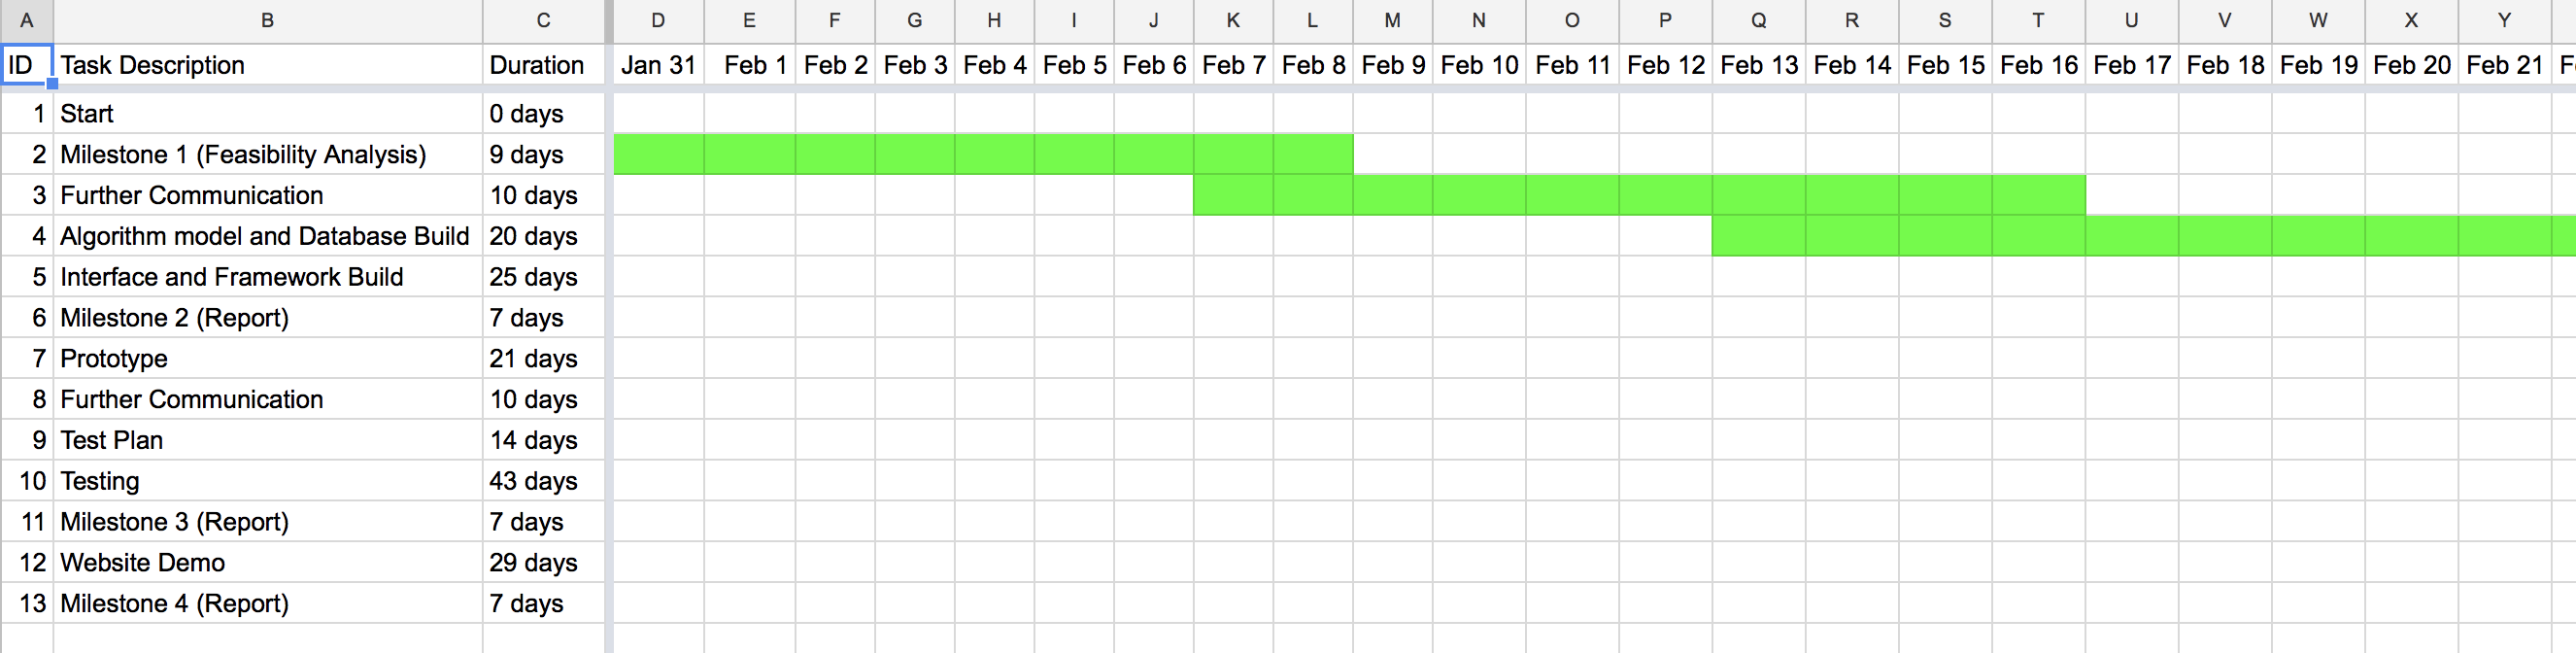
\includegraphics[scale=0.5,angle=270]{1.png}
\end{figure}

\hfill \break
\begin{figure}[ht]
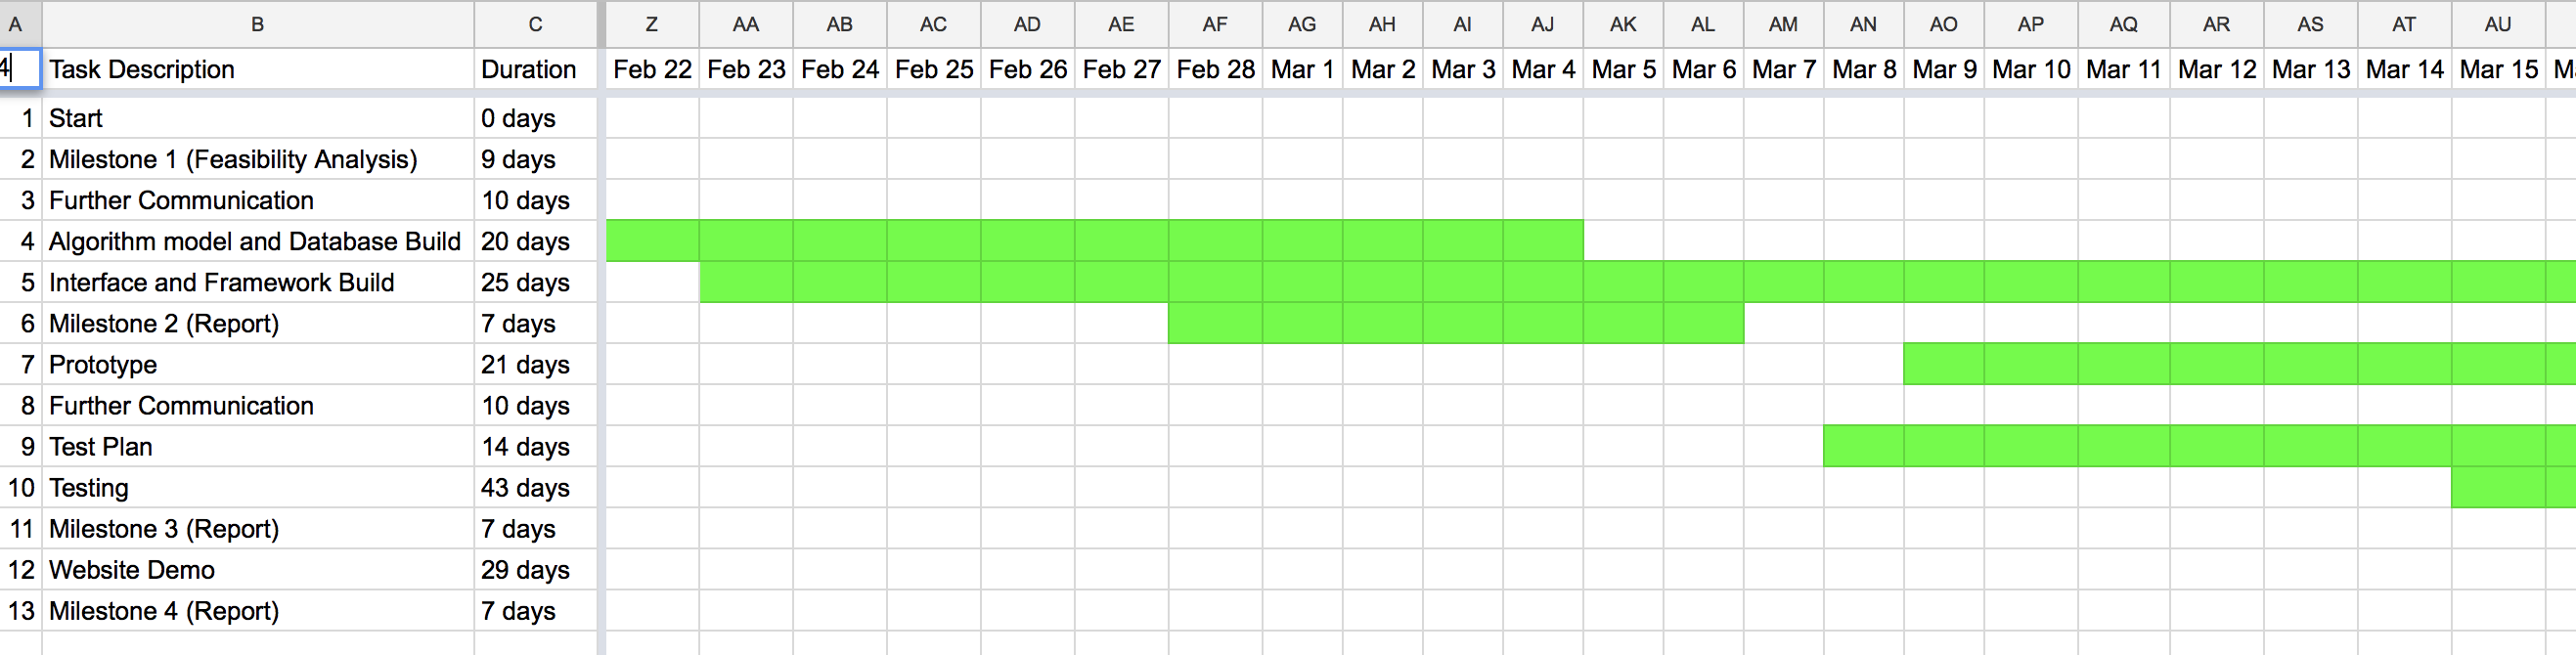
\includegraphics[scale=0.5,angle=270]{2.png}
\end{figure}

\hfill \break
\begin{figure}[ht]
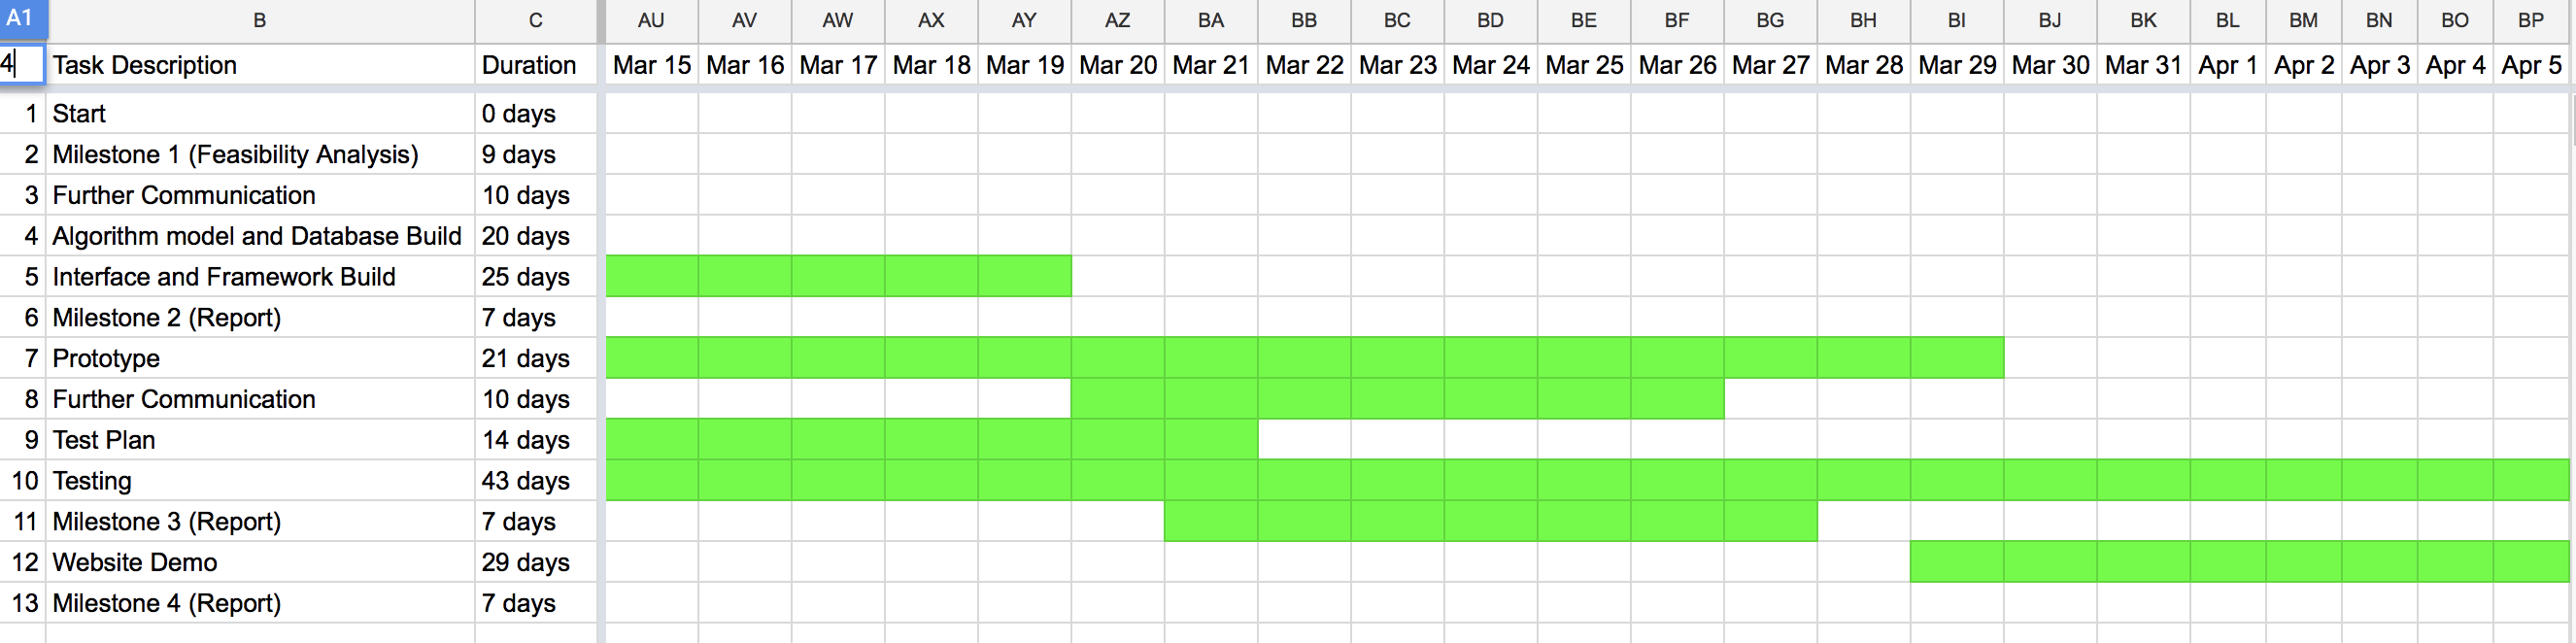
\includegraphics[scale=0.5,angle=270]{3.png}
\end{figure}

\hfill \break
\begin{figure}[ht]
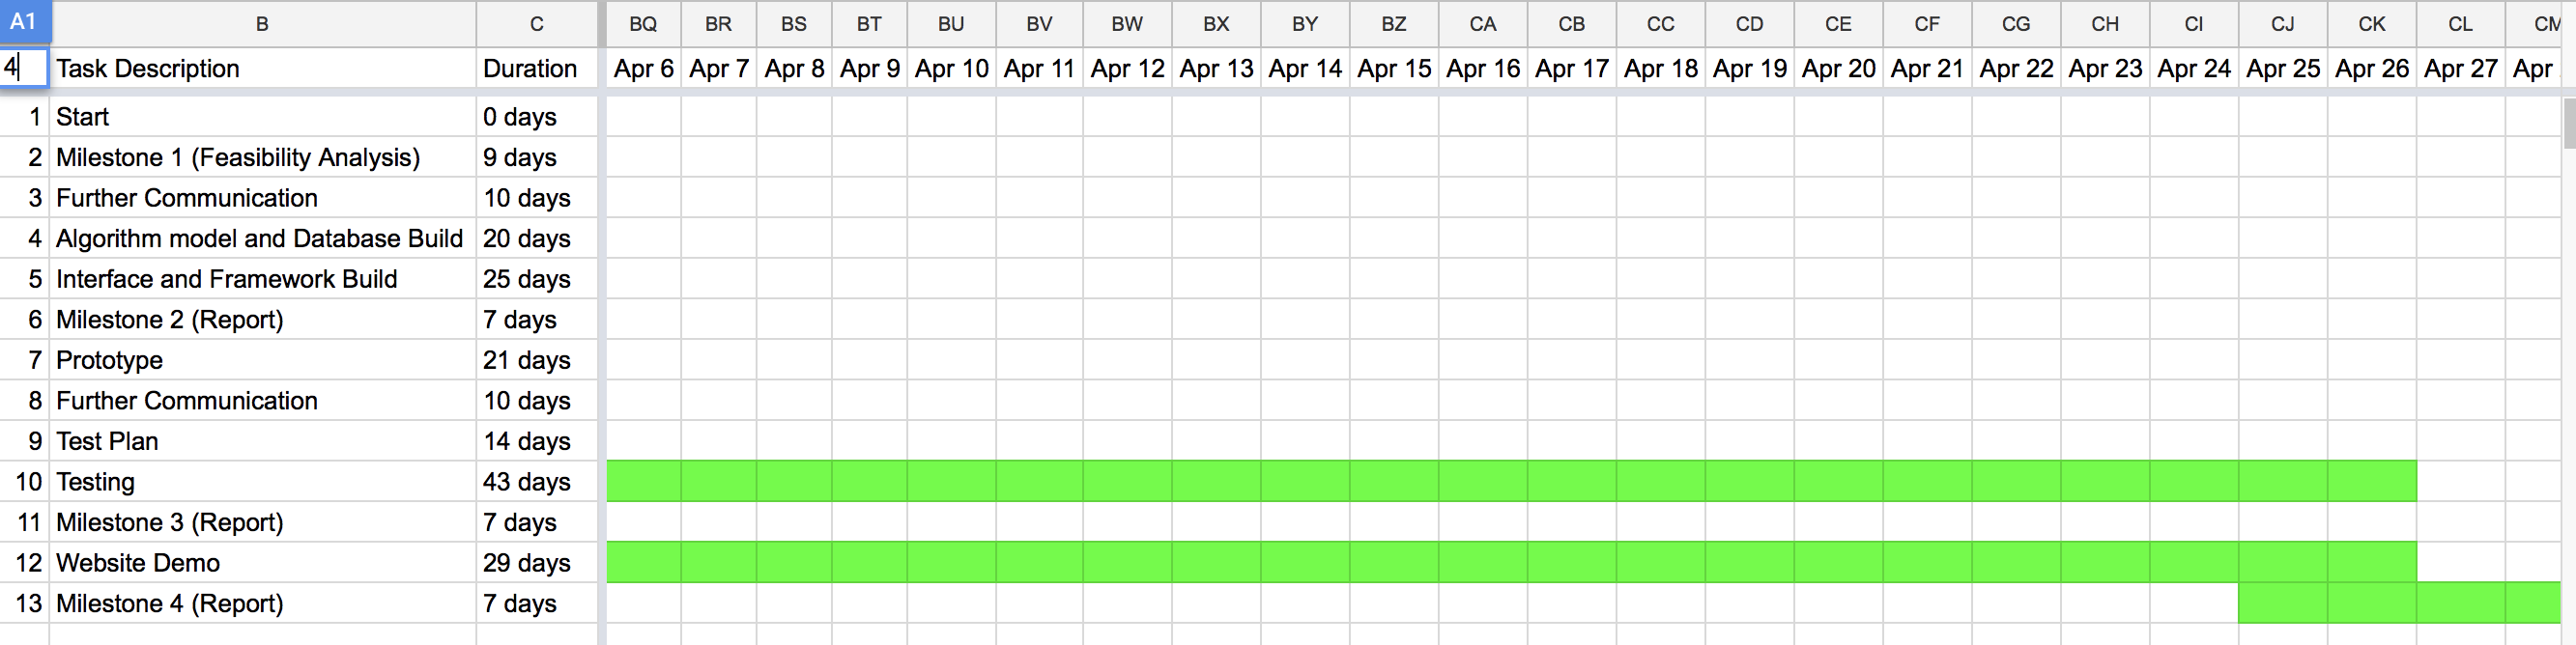
\includegraphics[scale=0.5,angle=270]{4.png}
\end{figure}

\hfill \break
\begin{figure}[ht]
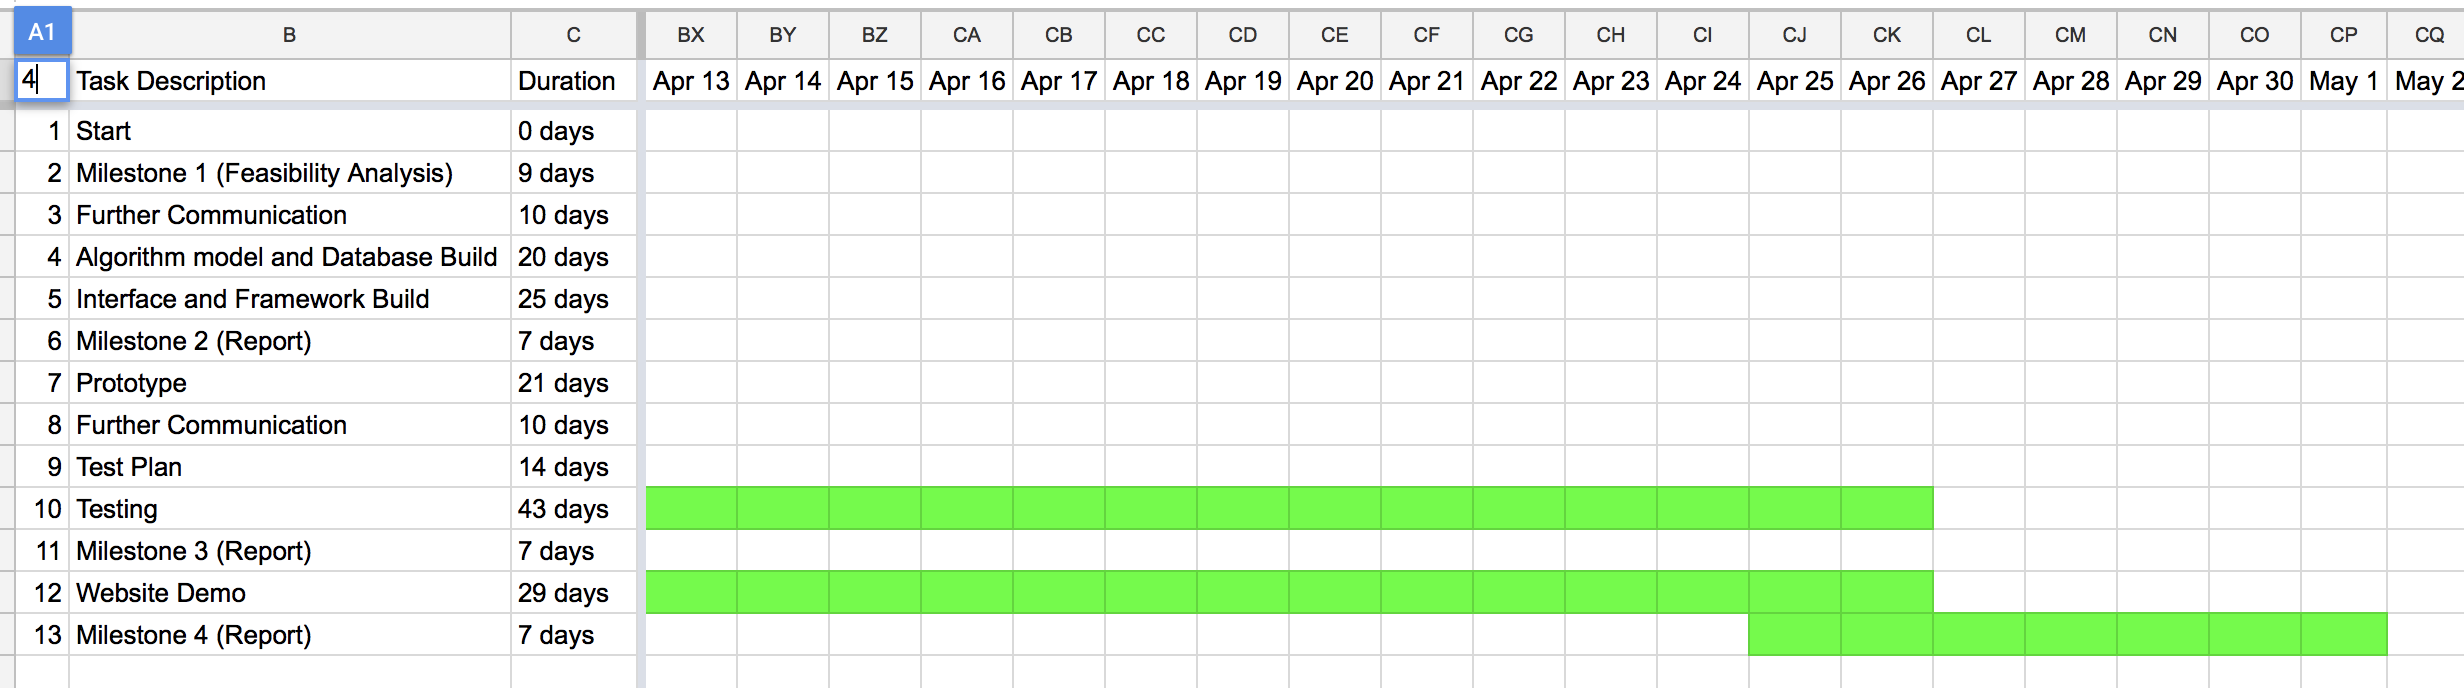
\includegraphics[scale=0.5,angle=270]{5.png}
\end{figure}

\end{document}
